\documentclass[10pt]{article}
\usepackage[left=1.5cm,top=1.5cm,right=1.5cm,bottom=1.5cm]{geometry}

\usepackage{mathtools}
\usepackage{amsmath}
\usepackage{amssymb}
\usepackage{relsize}
\DeclareMathSizes{10}{12}{7}{5}

\usepackage{polski}
\usepackage{indentfirst}
\usepackage{fontspec}
\usepackage{setspace}
\setmainfont{Verdana}
\thispagestyle{empty}

\begin{document}
\setlength{\parindent}{0cm}
\setstretch{1.3}

%\title{Laboratorium problemowe}
%\maketitle

\section*{Model matematyczny suwnicy}
\subsection*{Sformułowanie równań}
\begin{center}
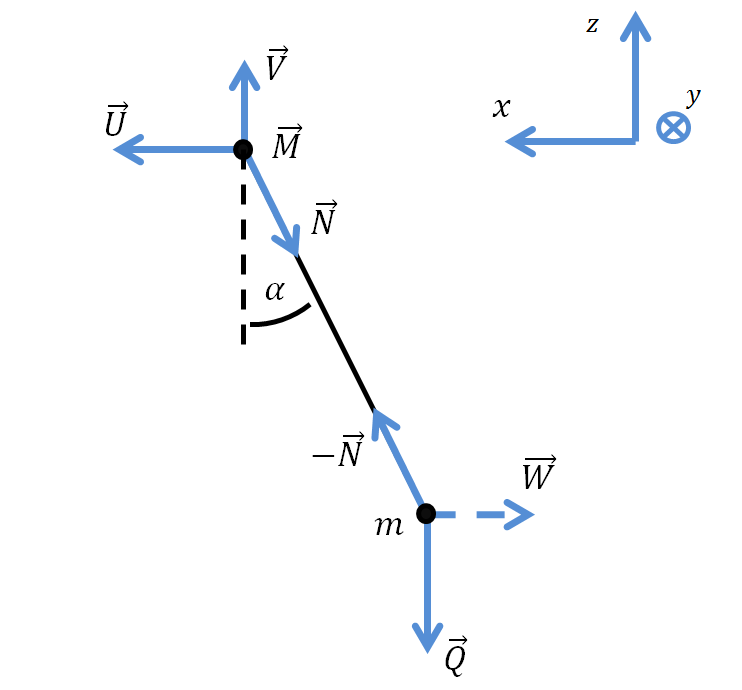
\includegraphics[width=9cm]{pic1}
\end{center}

Model opisać można za pomocą czterech równań. Pierwsze nich wynika z przedstawienia zależności między przyspieszeniem $\vec{a_M}$ wózka na suwnicy symbolizowanego przez masę $\vec{M}$ (powód użycia wektora został przedstawiony dalej), a odpowiednimi siłami, które na niego działają:
\begin{equation}
\vec{U} + \vec{V} + \vec{N} + \vec{B} = \vec{M} \otimes \vec{a_M}
\end{equation}

gdzie:

\begin{description}
\item[$\vec{U} = \begin{bmatrix} u_x & u_y & 0 \end{bmatrix}^T$] - sygnał sterujący (siła)
\item[$\vec{V} = \begin{bmatrix} 0 & 0 & v_z \end{bmatrix}^T$] - pionowa składowa siły reakcji prowadnicy
\item[$\vec{N} = \begin{bmatrix} n_x & n_y & n_z \end{bmatrix}^T$] - siła naciągu liny
\item[$\vec{B} = \begin{bmatrix} b_x (\dot{x_M}) & b_y (\dot{y_M}) & 0 \end{bmatrix}^T$] - wypadkowa siła tarć i innych oporów mechanicznych
\item[$\begin{bmatrix} x_M & y_M & z_M \end{bmatrix}^T$] - położenie wózka
\item[$\vec{a_M} = \begin{bmatrix} \ddot{x_M} & \ddot{y_M} & 0 \end{bmatrix}^T$] - przyspieszenie wózka
\item[$\begin{bmatrix} a_1 & ... & a_n \end{bmatrix}^T \otimes \begin{bmatrix} b_1 & ... & b_n \end{bmatrix}^T \stackrel{\text{def}}{=} \begin{bmatrix} a_1b_1 & ... & a_n b_n \end{bmatrix}^T$] - iloczyn wektorowy "po współrzędnych"
\item[$\vec{M} = \begin{bmatrix} m_C & m_C + m_F & 0 \end{bmatrix}$] - masa wózka i ramy; zastosowany został wektor w miejsce skalarnej wielkości, aby rozróżnić sytuację, gdy poruszany jest tylko wózek (ruch wzdłuż współrzędnej $x$), a gdy poruszany jest wózek wraz z jego prowadnicą (wzdłuż współrzędnej $y$); zakładamy brak ruchu wzdłuż współrzednej $z$, więc ta składowa wektora jest równa $0$
\item[$m_C$] - masa wózka
\item[$m_F$] - masa prowadnicy wózka
\end{description}

Drugie równanie wynika z zależności między przyspieszeniem $\vec{a_m}$ obciążenia (symbolizowanego przez masę $m$), a odpowiednimi siłami, które na to obciążenie oddziałują. Wspomniane przyspieszenie jest wyznaczane względem wózka, więc analizowany układ odniesienia jest układem inercjalnym, który poddany jest przyspieszeniu $\vec{a_M}$:
\begin{equation}
\vec{Q} + \vec{W} - \vec{N} = m\vec{a_m}
\end{equation}

gdzie:
\begin{description}
\item[$\vec{Q} = \begin{bmatrix} 0 & 0 & -mg \end{bmatrix}^T$] - siła grawitacji działająca na obciążenie
\item[$\vec{W} = -m\vec{a_M}$] - siła bezwładności wynikająca z inercjalności układu odniesienia
\item[$m$] - masa obciążenia
\item[$\vec{a_m} = \begin{bmatrix} \ddot{x_m} & \ddot{y_m} & \ddot{z_m} \end{bmatrix}^T$] - przyspieszenie obciążenia w inercjalnym układzie odniesienia
\end{description}

Z braku ruchu wzdłuż prostej prowadzącej przez położenia wózka i obciążenia w analizowanym inercjalnym układzie odniesienia, a także biorąc pod uwagę fakt, że siła $\vec{N}$ musi być równoległa do tej prostej, wynika trzecie równanie:
\begin{equation}
\vec{N} = \begin{bmatrix} sin(\alpha_x) \\ sin(\alpha_y) \\ -cos(\alpha) \end{bmatrix}
\big( |\vec{Q}|cos(\alpha) + |\vec{W}|sin(\alpha) \big)
\end{equation}

Rozmieszczenie kątów $\alpha_x$, $\alpha_y$ i $\alpha$ zostało przestawione na rysunku poniżej:
\begin{center}
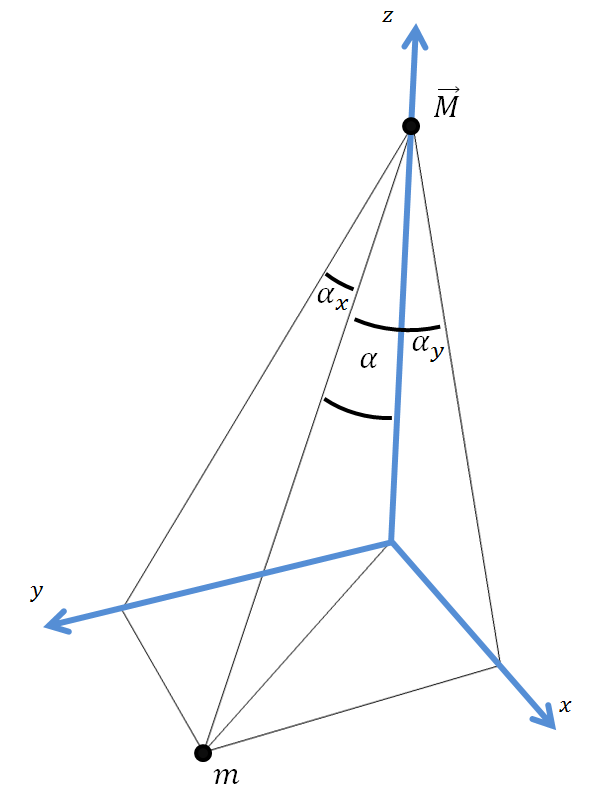
\includegraphics[width=9cm]{pic2mod}
\end{center}

Zauważyć też można zależność między kątami:
\begin{equation}
sin^2(\alpha_x) + sin^2(\alpha_y) = sin^2(\alpha)
\end{equation}

Po podstawieniu równania (3) oraz wszystkich pozostałych wartości do równań (1) i (2) uzyskany zostaje następujący układ równań:
\begin{equation}
\begin{bmatrix} u_x \\ u_y \\ 0 \end{bmatrix} + 
\begin{bmatrix} 0 \\ 0 \\ v_z \end{bmatrix} +
\begin{bmatrix} sin(\alpha_x) \\ sin(\alpha_y) \\ -cos(\alpha) \end{bmatrix}
\Bigg( |m\vec{g}|cos(\alpha) + m \Bigg| \begin{bmatrix} \ddot{x_M} \\ \ddot{y_M} \\ 0 \end{bmatrix} \Bigg| sin(\alpha) \Bigg) + 
\begin{bmatrix} b_x(\dot{x_M}) \\ b_y(\dot{y_M}) \\ 0 \end{bmatrix} = 
\begin{bmatrix} m_C \ddot{x_M} \\ (m_C + m_F) \ddot{y_M} \\ 0 \end{bmatrix}
\end{equation}
\begin{equation}
\begin{bmatrix} 0 \\ 0 \\ -mg \end{bmatrix} -
m \begin{bmatrix} \ddot{x_M} \\ \ddot{y_M} \\ 0 \end{bmatrix} - 
\begin{bmatrix} sin(\alpha_x) \\ sin(\alpha_y) \\ -cos(\alpha) \end{bmatrix}
\Bigg( |m\vec{g}|cos(\alpha) + m \Bigg| \begin{bmatrix} \ddot{x_M} \\ \ddot{y_M} \\ 0 \end{bmatrix} \Bigg| sin(\alpha) \Bigg)
 = m\vec{a_m}
\end{equation}

Z równań usunąć można równania dla składowej $z$, gdyż nie są one potrzebne dla dalszej analizy. Po dodatkowych uproszczeniach:

\begin{equation}
\begin{bmatrix} u_x \\ u_y \end{bmatrix} + 
m \begin{bmatrix} sin(\alpha_x) \\ sin(\alpha_y) \end{bmatrix}
\Bigg( g \cdot cos(\alpha) + \Bigg| \begin{bmatrix} \ddot{x_M} \\ \ddot{y_M} \end{bmatrix} \Bigg| sin(\alpha) \Bigg) + 
\begin{bmatrix} b_x(\dot{x_M}) \\ b_y(\dot{y_M}) \end{bmatrix} = 
\begin{bmatrix} m_C \ddot{x_M} \\ (m_C + m_F) \ddot{y_M} \end{bmatrix}
\end{equation}
\begin{equation}
 - \begin{bmatrix} \ddot{x_M} \\ \ddot{y_M} \end{bmatrix} - 
\begin{bmatrix} sin(\alpha_x) \\ sin(\alpha_y) \end{bmatrix}
\Bigg( g \cdot cos(\alpha) + \Bigg| \begin{bmatrix} \ddot{x_M} \\ \ddot{y_M} \end{bmatrix} \Bigg| sin(\alpha) \Bigg)
 = \vec{a_m}
\end{equation}

Biorąc pod uwagę, że w rzeczywistym modelu nie ma możliwości pomiaru liniowych przesunięć, prędkości ani przyspieszeń obciążenia, konieczne jest wyrażenie przyspieszenia $\vec{a_m}$ przy pomocy kątów $\alpha_x$ i $\alpha_y$ oraz długości liny $l$. Położenie względne obciążenia wyrazić można wzorem:
\begin{equation}
\vec{x_m} = l \begin{bmatrix} sin(\alpha_x) \\ sin(\alpha_y) \end{bmatrix}
\end{equation}

Przyspieszenie będzie zatem wyrażone wzorem:
\begin{equation}
\vec{a_m} = l
\begin{bmatrix}
\ddot{\alpha_x} cos(\alpha_x) - (\dot{\alpha_x})^2 sin(\alpha_x) \\
\ddot{\alpha_y} cos(\alpha_y) - (\dot{\alpha_y})^2 sin(\alpha_y)
\end{bmatrix}
\end{equation}

Po podstawieniu zależności (10) do równania (8) i przyrównaniu poszczególnych składowych równań (7) i (8) otrzymany zostaje następujący układ równań:

\begin{equation}
u_x + mg \cdot sin(\alpha_x) cos(\alpha) + m \cdot sin(\alpha_x) \sqrt{(\ddot{x_M})^2 + (\ddot{y_M})^2)} + b_x(\dot{x_M}) = m_C \ddot{x_M}
\end{equation}
\begin{equation}
u_y + mg \cdot sin(\alpha_y) cos(\alpha) + m \cdot sin(\alpha_y) \sqrt{(\ddot{x_M})^2 + (\ddot{y_M})^2)} + b_y(\dot{y_M}) = (m_C + m_F) \ddot{y_M}
\end{equation}
\begin{equation}
-\ddot{x_M}-sin(\alpha_x) \Big( g \cdot cos(\alpha) + sin(\alpha)\sqrt{(\ddot{x_M})^2 + (\ddot{y_M})^2)} \Big) = l \big( \ddot{\alpha_x} cos(\alpha_x) - (\dot{\alpha_x})^2 sin(\alpha_x) \big)
\end{equation}
\begin{equation}
-\ddot{y_M}-sin(\alpha_y) \Big( g \cdot cos(\alpha) + sin(\alpha)\sqrt{(\ddot{x_M})^2 + (\ddot{y_M})^2)} \Big) = l \big( \ddot{\alpha_y} cos(\alpha_y) - (\dot{\alpha_y})^2 sin(\alpha_y) \big)
\end{equation}

\newpage
\subsection*{Zastosowanie obliczeń numerycznych do wyznaczenia rozwiązań}
Aby możliwe było zastosowanie obliczeń numerycznych do powyższego modelu, konieczne jest przekształcenie powyższych równań, do takich postaci, aby drugie pochodne zmiennych stanu ($\ddot{x_M}, \ddot{y_M}, \ddot{\alpha_x}, \ddot{\alpha_y}$) były wyrażone w zależności od pozostałych zmiennych. W przypadku przyspieszeń kątowych, przekształcenie to jest proste, gdyż sprowadza się do drobnych przekształceń równań 13 i 14:
\begin{equation}
\ddot{\alpha_x} = \frac{1}{l \cdot cos(\alpha_x)} \bigg(l (\dot{\alpha_x})^2 sin(\alpha_x) - \ddot{x_M}-sin(\alpha_x) \Big( g \cdot cos(\alpha) + sin(\alpha)\sqrt{(\ddot{x_M})^2 + (\ddot{y_M})^2)} \Big) \bigg)
\end{equation}
\begin{equation}
\ddot{\alpha_y} = \frac{1}{l \cdot cos(\alpha_y)} \bigg(l (\dot{\alpha_y})^2 sin(\alpha_y) - \ddot{y_M}-sin(\alpha_y) \Big( g \cdot cos(\alpha) + sin(\alpha)\sqrt{(\ddot{x_M})^2 + (\ddot{y_M})^2)} \Big) \bigg)
\end{equation}

W przypadku przyspieszeń liniowych sprawa jest jednak bardziej skompilowana, gdyż konieczne jest rozwiązanie układu równań o postaci (ze względu na niewiadome $X$ i $Y$):
\begin{equation}
\begin{cases}
A_1+B_1\sqrt{X^2 + Y^2} = C_1X \\ 
A_2+B_2\sqrt{X^2 + Y^2} = C_2Y
\end{cases}, \quad C_1 > 0, \quad C_2 > 0
\end{equation}

\subsection*{Rozwiązanie układu równań (17)}
Po prostych przekształceniach można zauważyć afiniczną zależność między niewiadomymi:
\begin{equation}
\begin{cases}
B_1 B_2 \sqrt{X^2 + Y^2} = C_1 B_2 X - A_1 B_2 \\ 
B_1 B_2 \sqrt{X^2 + Y^2} = C_2 B_1 Y - A_2 B_1
\end{cases}
\end{equation}
\begin{equation}
C_1 B_2 X - A_1 B_2 = C_2 B_1 Y - A_2 B_1
\end{equation}

Z drugiej strony, po podniesieniu na przykład pierwszego z równań (17) do kwadratu, możliwe jest zastosowanie tej zależności (19), aby sprowadzić zadanie do rozwiązania równania kwadratowego jednej niewiadomej:
\begin{equation}
C_2^2 B_1^2 Y^2 = C_2^2 (C_1 X - A_1)^2 - C_2^2 B_1^2 X^2
\end{equation}
\begin{equation}
(C_1 B_2 X - A_1 B_2 + A_2 B_1)^2 = C_2^2 (C_1 X - A_1)^2 - C_2^2 B_1^2 X^2
\end{equation}
\begin{equation}
\big(C_1^2 C_2^2 - C_2^2 B_1^2 - C_1^2 B_2^2 \big) X^2 + 
2\big(C_1B_2 (A_2B_1 - A_1B_2) - A_1C_1C_2^2 \big) X +
A_1^2 C_2^2 + \big(A_2B_1 - A_1B_2 \big)^2
 = 0
\end{equation}

Aby wyznaczyć wartość $Y$ konieczne jest rozwiązanie analogicznego równania kwadratowego:
\begin{equation}
\big(C_1^2 C_2^2 - C_2^2 B_1^2 - C_1^2 B_2^2 \big) Y^2 + 
2\big(C_2B_1 (A_1B_2 - A_2B_1) - A_2C_2C_1^2 \big) Y +
A_2^2 C_1^2 + \big(A_1B_2 - A_2B_1 \big)^2
 = 0
\end{equation}

\end{document}